\documentclass{article}
\usepackage{color}
\usepackage{tikz}
\usepackage{float}
\usepackage{tabularx}
\usepackage{amsmath}
\usepackage{amssymb}
\usepackage{listings}
\usepackage{enumitem}
\usepackage{syntax}
\usepackage{csquotes}
\usepackage{pgfplots}
%\usepackage[backend=biber]{biblatex}
%\addbibresource{references.bib}


\definecolor{dkgreen}{rgb}{0,0.6,0}
\definecolor{gray}{rgb}{0.5,0.5,0.5}
\definecolor{mauve}{rgb}{0.58,0,0.82}
\definecolor{variables}{RGB}{126,25,121}
\definecolor{symbolred}{RGB}{178,34,34}


\lstdefinelanguage{eprime}
{
	morekeywords={
		letting, be,
		indexed, by, of,
		given, 
		find,
		maximising, minimising,
		such, that,
		max, min,
		sum,
		forall, forAll, exists, alldifferent, table
	},
	morecomment=[l]{\$},
}

\lstset{
  language={eprime},
  frame=tb,
  alsoletter={\\}.:+-<>{/},
  emph = [1]{int, bool, matrix, domain},
  emphstyle = [1]{\color{variables}},
  emph = [2]{:, +, -, ., .., *, \%, /\\, \\/, <, >, =},
  emphstyle = [2]{\color{symbolred}},  
  numbers=left,
  stepnumber=1,
  aboveskip=3mm,
  belowskip=3mm,
  showstringspaces=false,
  columns=flexible,
  basicstyle={\small\ttfamily},
  numberstyle=\color{gray},
  keywordstyle=\color{blue},
  commentstyle=\color{dkgreen},
  stringstyle=\color{mauve},
  breaklines=true,
  breakatwhitespace=true,
  tabsize=4,
  moredelim=**[is][\color{red}]{@}{@},  
}

\setlength{\grammarindent}{12em}

%\renewcommand{\lstlistingname}{Algorithm}
%\newcommand{\tablerow}[4]{ #1 & #2 & #3 & #4\\}
\newcommand{\n}[0]{\\[\baselineskip]}

%%%%
 % Macro for creating title page
 % #1 - Module code/name
 % #2 - Lecturer
%%%%
\newcommand{\maketitlepage}[2]{
\begin{titlepage}
	\centering
    \includegraphics[scale = 0.4]{01-standard-vertical-black.png}\\	% University Logo
	\textsc{\LARGE #1}\\[0.5 cm]				% Course Code
	\rule{\linewidth}{0.2 mm} \\[0.4 cm]
	{ \huge \bfseries \thetitle}
	\rule{\linewidth}{0.2 mm} \\[0.5 cm]
	\textsc{\large \thedate}\\[1.5 cm]
	
	\begin{minipage}{0.4\textwidth}
		\begin{flushleft} \large
			\emph{Lecturer:}\\
			#2
			\end{flushleft}
			\end{minipage}
			\begin{minipage}{0.4\textwidth}
            
			\begin{flushright} \large
			\emph{Submitted By:} \\
			\theauthor
		\end{flushright}
        
	\end{minipage}\\
	
\end{titlepage}
}

\title{The Bombastic Modelling Problem}
\author{140011146}

\makeatletter
\let\thetitle\@title
\let\theauthor\@author
\let\thedate\@date
\makeatother

\begin{document}

\maketitlepage{CS4402 Constraint Programming}{Ian Miguel}




\section{Introduction}

\section{Design and Implementation}
\subsection{Initial states}
There are three sets of state variables that need to be set up as the initial states: the avatar's position, the locations of the blocks and the cells of the grid. 

\begin{lstlisting}
$ Avatar's initial position
avatarCurrentRow[0] = avatarInitRow,
avatarCurrentCol[0] = avatarInitCol,

$ Initial locations for blocks
forall block : int(1..numBlocks) .
    blocksCurrentRow[0,block] = blocksInitRow[block] /\
    blocksCurrentCol[0,block] = blocksInitCol[block],

$ Initial cells of grid
forall row : int(1..r) .
    forall col : int(1..c) .
        gridCurrent[0,row,col] = gridInit[row,col],
\end{lstlisting}

\subsection{Invalid states}
Next are the constraints for invalid states of the game. This restricts the model to not have states such as having the avatar and a block be in the same position. 

\begin{lstlisting}

\end{lstlisting}

\subsection{Movement}

\subsection{Grid}

\section{Results}


\begin{figure}[H]
\centering
\begin{minipage}{0.4\textwidth}
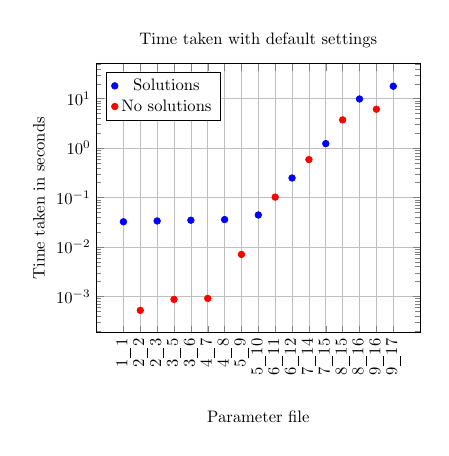
\begin{tikzpicture}[scale=0.6]
\begin{axis}[
	title={Time taken with default settings},
	ylabel={Time taken in seconds},
	ymode=log,
	xlabel={Parameter file},
	x label style={yshift=-0.5cm},
	xtick={1,2,3,4,5,6,7,8,9,10,11,12,13,14,15,16,17},
	xticklabels={1_1, 2_2, 2_3, 3_5, 3_6, 4_7, 4_8, 5_9, 5_10, 6_11, 6_12, 7_14, 7_15, 8_15, 8_16, 9_16, 9_17},
	x tick label style={rotate=90, anchor=east},
	ymajorgrids=true,
	xmajorgrids=true,
	legend pos=north west,
	]

\addplot[only marks, color=blue, mark=*,] coordinates { (1,0.032255) (3,0.03346) (5,0.034649) (7,0.035724) (9,0.044199) (11,0.247985) (13,1.2295) (15,9.8467) (17,17.8504)};
\label{plot:solution-time}
\addlegendentry{Solutions}

\addplot[only marks, color=red, mark=*,] coordinates { (2,0.000519) (4,0.000865) (6,0.000906) (8,0.007035) (10,0.10165) (12,0.585305) (14,3.72043) (16,6.11084)};
\label{plot:nosolution-time}
\addlegendentry{No solutions}

\end{axis}
\end{tikzpicture}
\end{minipage}
%
\begin{minipage}{0.4\textwidth}
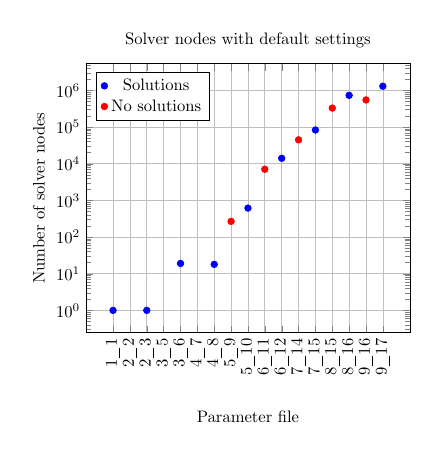
\begin{tikzpicture}[scale=0.6]
\begin{axis}[
	title={Solver nodes with default settings},
	ylabel={Number of solver nodes},
	ymode=log,
	xlabel={Parameter file},
	x label style={yshift=-0.5cm},
	xtick={1,2,3,4,5,6,7,8,9,10,11,12,13,14,15,16,17},
	xticklabels={1_1, 2_2, 2_3, 3_5, 3_6, 4_7, 4_8, 5_9, 5_10, 6_11, 6_12, 7_14, 7_15, 8_15, 8_16, 9_16, 9_17},
	x tick label style={rotate=90, anchor=east},
	ymajorgrids=true,
	xmajorgrids=true,
	legend pos=north west,
]

\addplot[only marks, color=blue, mark=*,] coordinates { (1,1) (3,1) (5,19) (7,18) (9,615) (11,14036) (13,82920) (15,730243) (17,1295303) };
\label{plot:solution-node}
\addlegendentry{Solutions}

\addplot[only marks, color=red, mark=*,] coordinates { (2,0) (4,0) (6,0) (8,267) (10,7052) (12,44769) (14,328133) (16,547164) };
\label{plot:nosolution-node}
\addlegendentry{No solutions}

\end{axis}
\end{tikzpicture}
\end{minipage}
\caption{Time taken and number of solver nodes for all given parameters}
\end{figure}



\begin{figure}[H]

\end{figure}

\subsection{Optimisations}

\subsection{Heuristics}

\begin{figure}[H]
\centering
\begin{minipage}{0.4\textwidth}
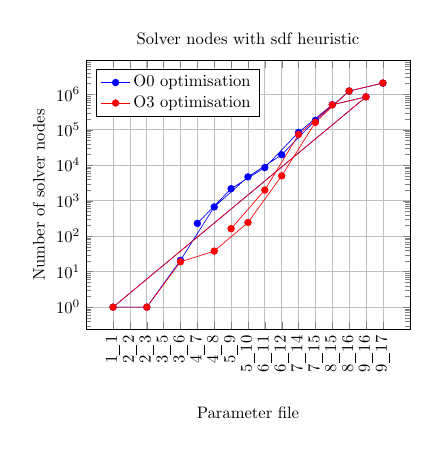
\begin{tikzpicture}[scale=0.6]
\begin{axis}[
	title={Solver nodes with sdf heuristic},
	ylabel={Number of solver nodes},
	ymode=log,
	xlabel={Parameter file},
	x label style={yshift=-0.5cm},
	xtick={1,2,3,4,5,6,7,8,9,10,11,12,13,14,15,16,17},
	xticklabels={1_1, 2_2, 2_3, 3_5, 3_6, 4_7, 4_8, 5_9, 5_10, 6_11, 6_12, 7_14, 7_15, 8_15, 8_16, 9_16, 9_17},
	x tick label style={rotate=90, anchor=east},
	ymajorgrids=true,
	xmajorgrids=true,
	legend pos=north west,
	]

\addplot[color=blue, mark=*,] coordinates { (2,0) (4,0) (6,229) (8,2184) (10,8579) (12,84300) (14,507126) (16,844406) (1,1) (3,1) (5,21) (7,668) (9,4688) (11,19720) (13,183603) (15,1230659) (17,2055840)};
\label{plot:sdf-o0}
\addlegendentry{O0 optimisation}

\addplot[color=red, mark=*,] coordinates { (2,0) (4,0) (6,0) (8,163) (10,1994) (12,73418) (14,502477) (16,841628) (1,1) (3,1) (5,19) (7,38) (9,243) (11,5021) (13,162024) (15,1239351) (17,2077990)};
\label{plot:sdf-o3}
\addlegendentry{O3 optimisation}

\end{axis}
\end{tikzpicture}
\end{minipage}
%
\begin{minipage}{0.4\textwidth}
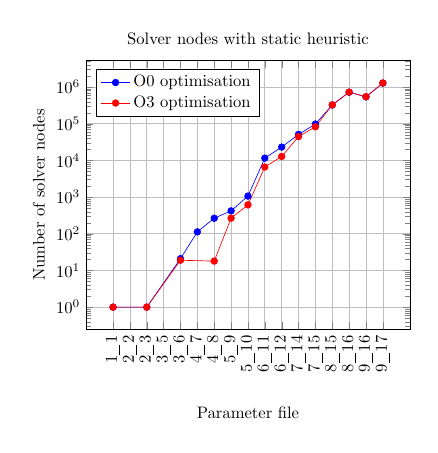
\begin{tikzpicture}[scale=0.6]
\begin{axis}[
	title={Solver nodes with static heuristic},
	ylabel={Number of solver nodes},
	ymode=log,
	xlabel={Parameter file},
	x label style={yshift=-0.5cm},
	xtick={1,2,3,4,5,6,7,8,9,10,11,12,13,14,15,16,17},
	xticklabels={1_1, 2_2, 2_3, 3_5, 3_6, 4_7, 4_8, 5_9, 5_10, 6_11, 6_12, 7_14, 7_15, 8_15, 8_16, 9_16, 9_17},
	x tick label style={rotate=90, anchor=east},
	ymajorgrids=true,
	xmajorgrids=true,
	legend pos=north west,
]

\addplot[color=blue, mark=*,] coordinates { (1,1) (2,0) (3,1) (4,0) (5,21) (6,113) (7,266) (8,422) (9,1068) (10,11586) (11,23143) (12,51454) (13,98558) (14,324862) (15,725870) (16,542821) (17,1287730) };
\label{plot:static-o0}
\addlegendentry{O0 optimisation}

\addplot[color=red, mark=*,] coordinates { (1,1) (2,0) (3,1) (4,0) (5,19) (6,0) (7,18) (8,267) (9,615) (10,6622) (11,12838) (12,44769) (13,82920) (14,328133) (15,730243) (16,547164) (17,1295303) };
\label{plot:static-o3}
\addlegendentry{O3 optimisation}

\end{axis}
\end{tikzpicture}
\end{minipage}
\caption{Number of solver nodes for different heuristics}
\end{figure}

\subsection{Custom instances}


\section{Conclusion and evaluation}

%\printbibliography

\end{document}



